\documentclass[11pt]{article}
\usepackage[letterpaper,margin=.65in]{geometry}
% Shared font contract for manuscript text, math and figure labels.
% Matplotlib reads this preamble verbatim; do not use host-specific paths here.
\usepackage[T1]{fontenc}
\usepackage[utf8]{inputenc}
\usepackage{newtxtext,newtxmath}

\usepackage{graphicx,microtype,caption}
\usepackage[hidelinks]{hyperref}
\captionsetup{font=small,labelfont=normalfont}
\graphicspath{{figures/}}
\emergencystretch=2em
\hypersetup{pdftitle={Tessera figure atlas},pdfauthor={Zeyu Fu}}
\begin{document}\raggedbottom
\noindent{\Large Tessera\quad Figure 1}\hfill 11 October 2026\par\medskip
\begin{center}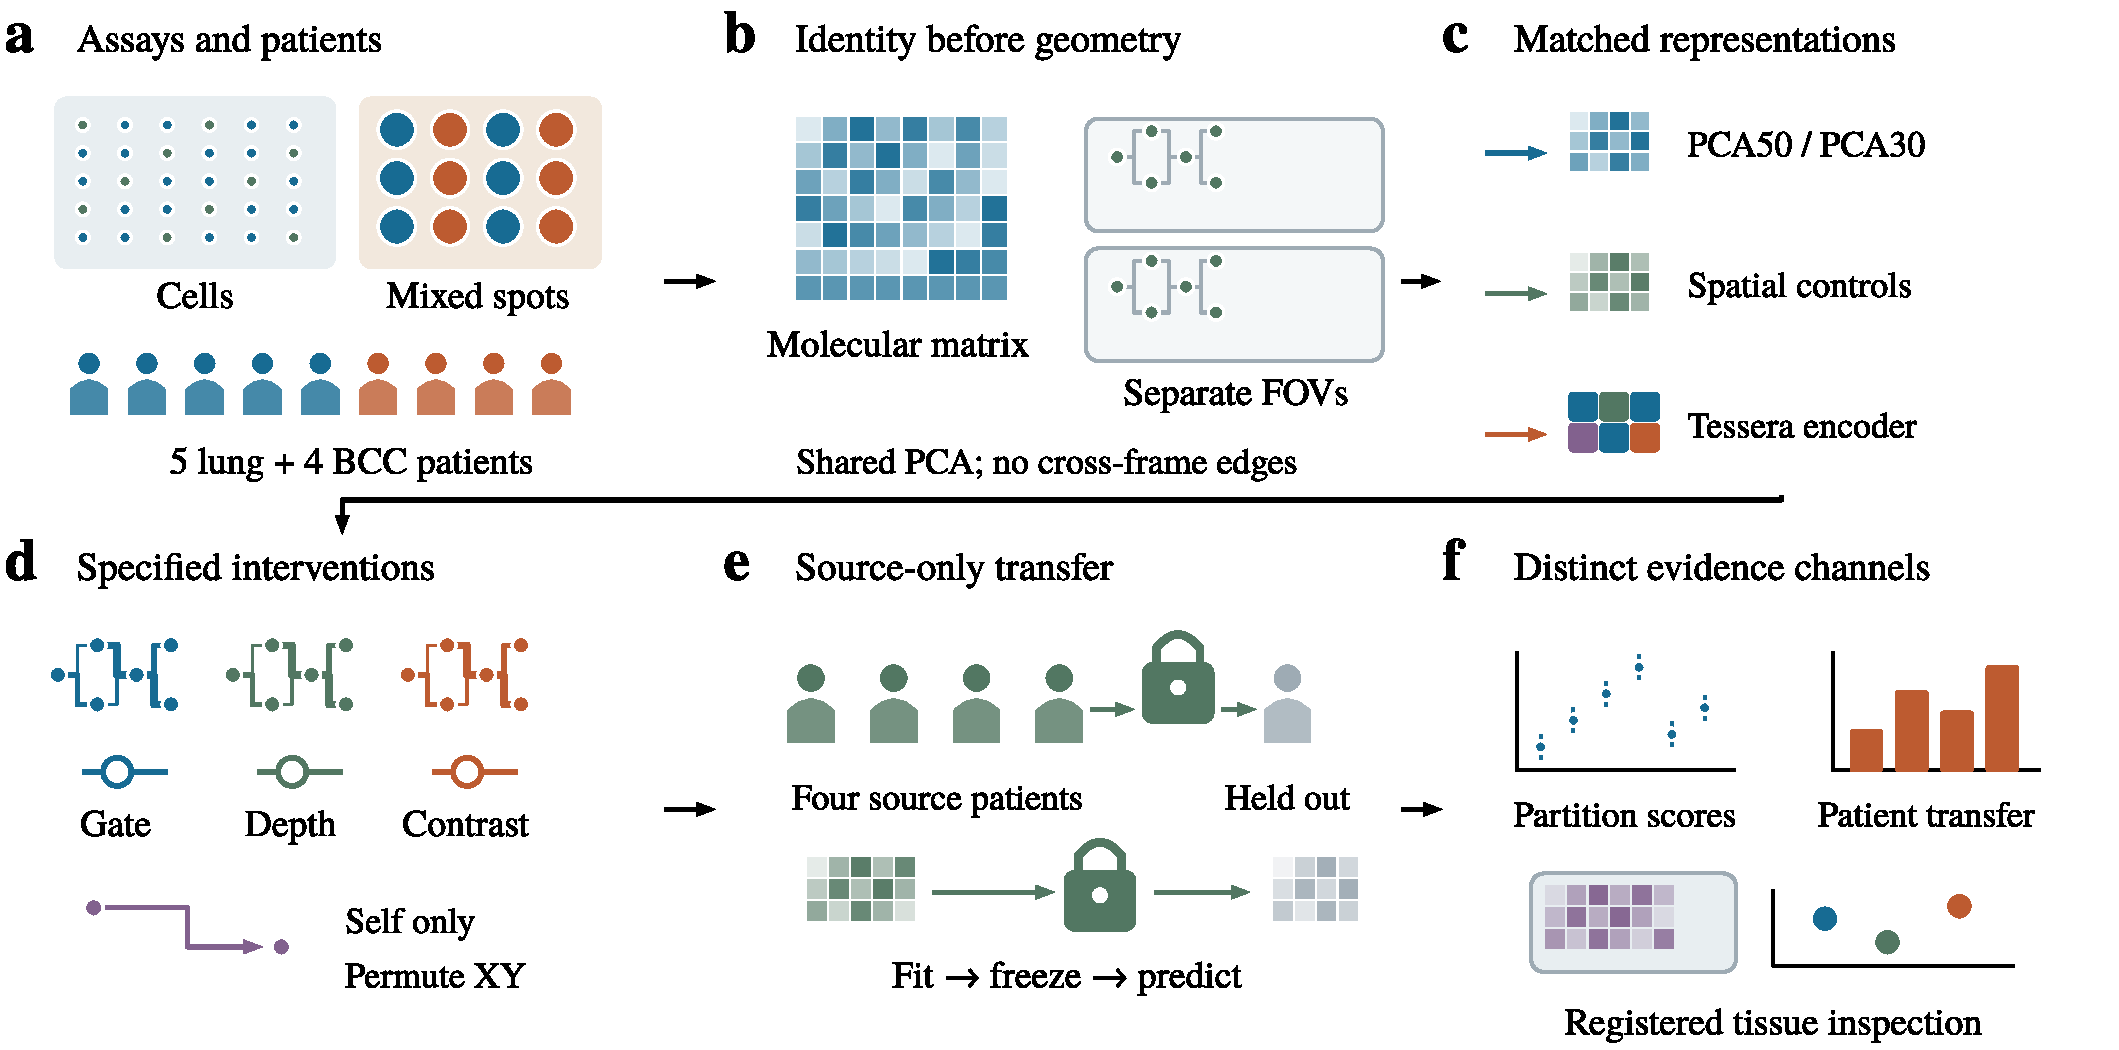
\includegraphics[width=\linewidth,height=.79\textheight,keepaspectratio]{figure01-workflow.pdf}\end{center}
\noindent{\small Figure 1. Study design. (a) Assays and independent patients. (b) Molecular matrices and separate coordinate frames enter one common preprocessing. (c) Expression-only, simple spatial and learned representations form matched branches. (d) Component removals change one part of the encoder at a time. (e) In patient transfer, four source patients fit every transformation and weight before the fifth patient is mapped. (f) Partition, transfer and tissue-inspection readouts are reported separately. Icons are conceptual.\par}
\clearpage
\noindent{\Large Tessera\quad Figure 2}\hfill 11 October 2026\par\medskip
\begin{center}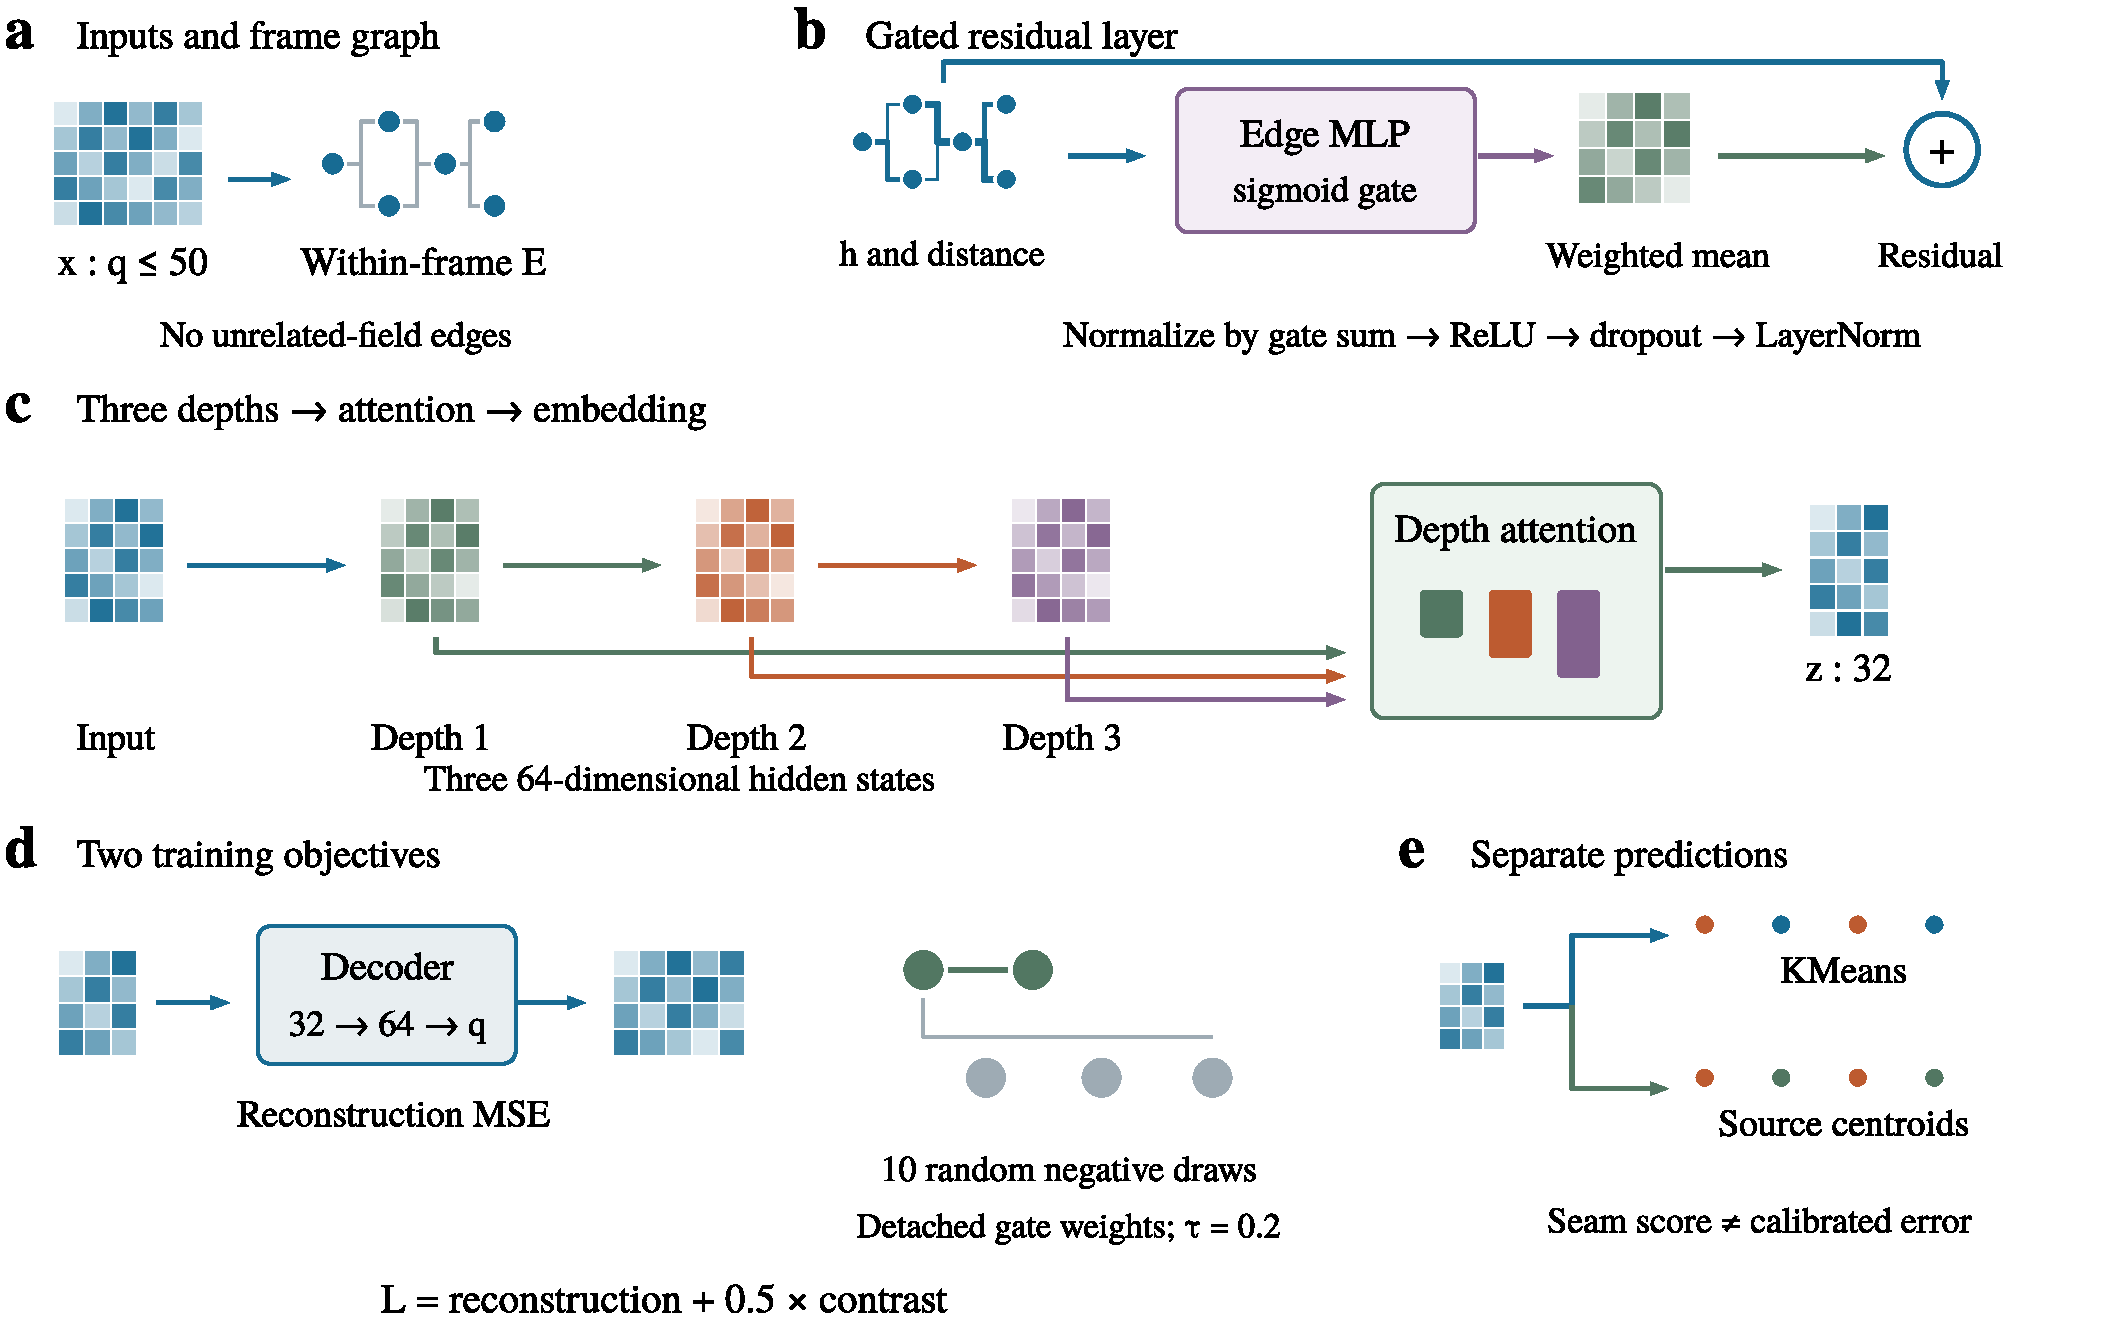
\includegraphics[width=\linewidth,height=.79\textheight,keepaspectratio]{figure13-architecture.pdf}\end{center}
\noindent{\small Figure 2. The Tessera computation as released. (a) Common PCA features and frame-restricted neighborhoods. (b) Edge differences and distances determine gates; gated messages are normalized before a residual update. (c) Three depths feed attention and a 32-dimensional projection. (d) A decoder reconstructs the PCA features; neighbor-positive contrast is weighted by detached gates. (e) K-means returns the within-object partition, and source-category centroids return transfer labels. Glyphs are conceptual; dimensions are those implemented.\par}
\clearpage
\noindent{\Large Tessera\quad Figure 3}\hfill 11 October 2026\par\medskip
\begin{center}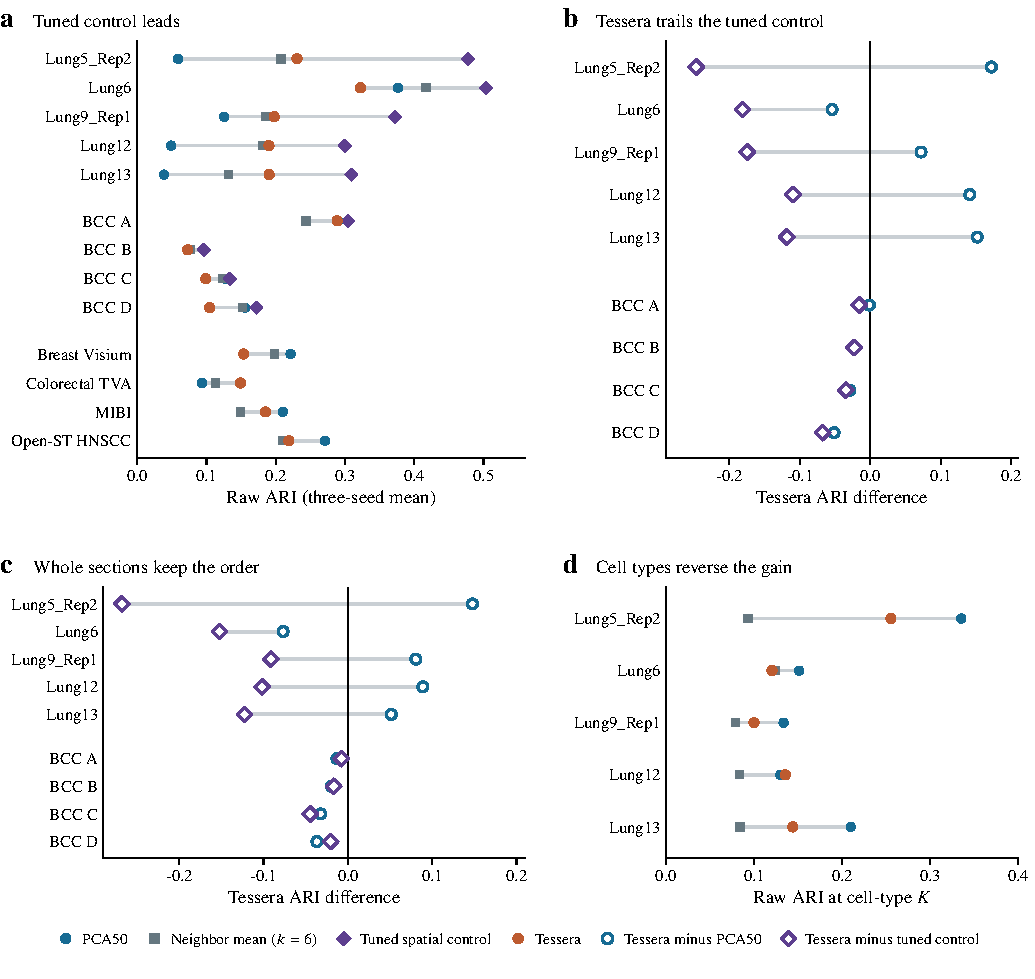
\includegraphics{figure03-comparison.pdf}\end{center}
\noindent{\small Figure 3. Tessera against expression-only, simple and tuned spatial controls. (a) Three-seed mean ARI per object; tuned controls are selected on other lung or BCC patients. (b) Bounded-field patient contrasts: Tessera minus PCA50 (open circles) and the nested control (open diamonds). (c) Uncapped whole-section sensitivity contrasts against PCA50 and fixed cohort-modal controls informed by the bounded analyses of the same patients. (d) Lung embeddings re-clustered at the cell-type cluster number and scored against supplied cell types.\par}
\clearpage
\noindent{\Large Tessera\quad Figure 4}\hfill 11 October 2026\par\medskip
\begin{center}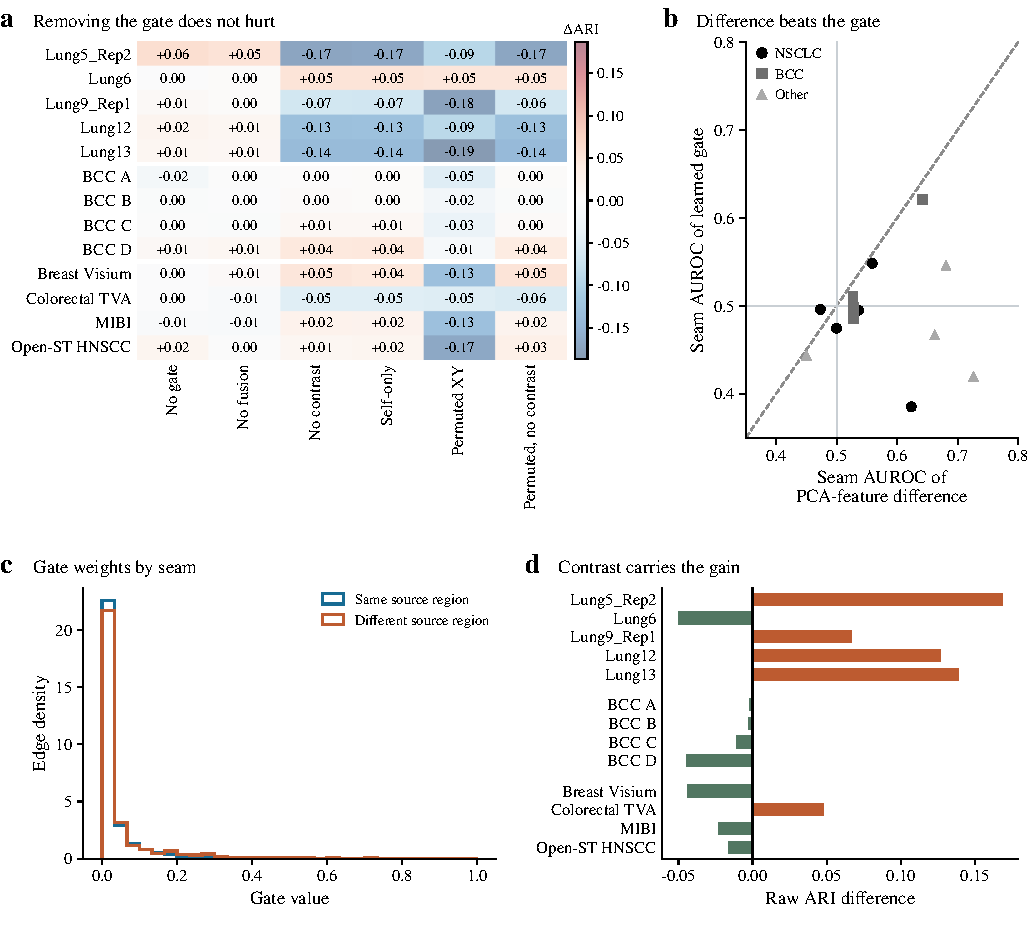
\includegraphics{figure04-ablations.pdf}\end{center}
\noindent{\small Figure 4. Which components carry the spatial effect. (a) Three-seed mean ARI of each control minus full Tessera; red favors the control. ``Permuted, no contrast'' trains on within-frame permuted coordinates without the contrastive term. (b) Seam discrimination by the last-layer gate versus by the plain PCA-feature difference on the same edges; points below the diagonal mean the gate is the weaker seam detector. (c) Last-layer gate distributions on edges within and across supplied regions in Lung5\_Rep2, seed 1. (d) Full Tessera minus the self-only encoder, the reference for the effect of measured geometry.\par}
\clearpage
\noindent{\Large Tessera\quad Figure 5}\hfill 11 October 2026\par\medskip
\begin{center}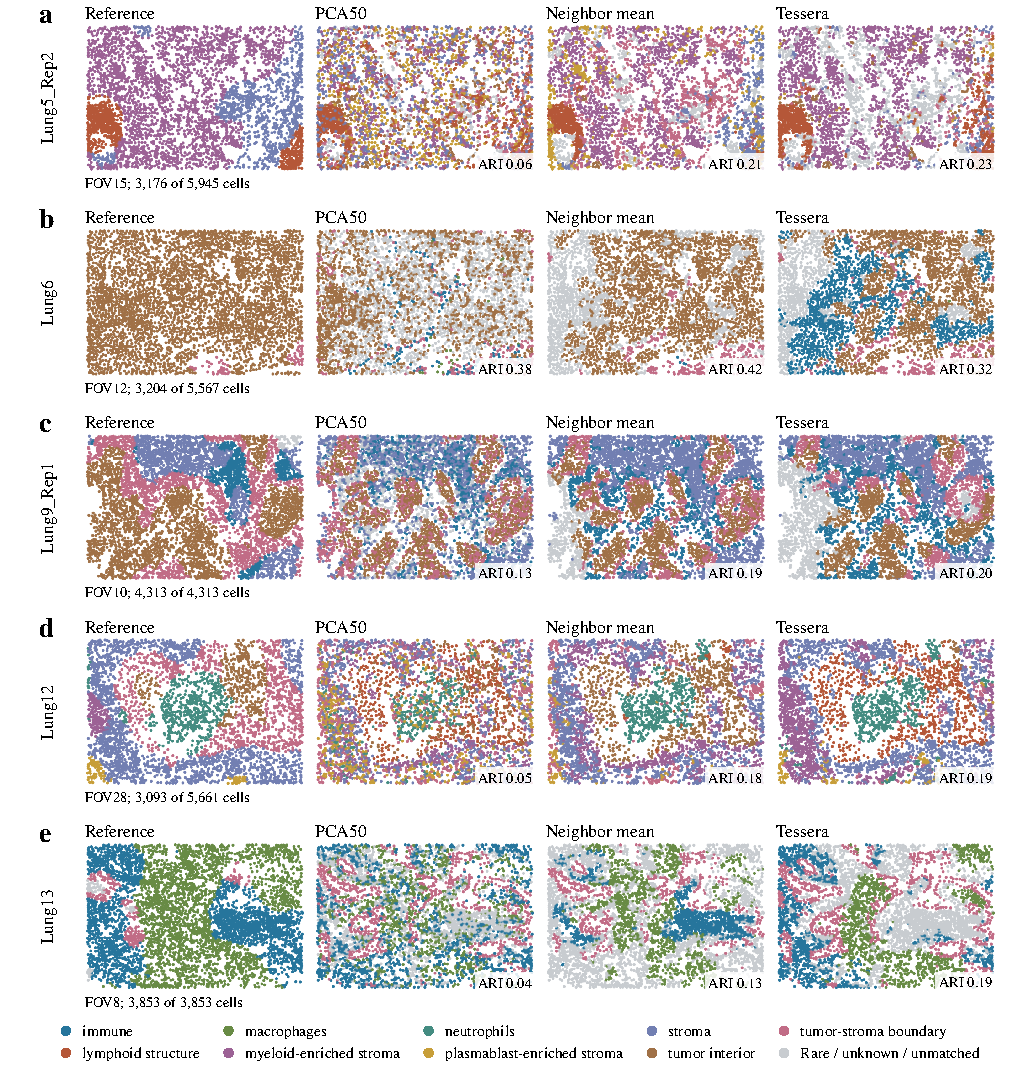
\includegraphics{figure05-nsclc-maps.pdf}\end{center}
\noindent{\small Figure 5. Lung display fields. Rows (a--e) show Lung5\_Rep2, Lung6, Lung9\_Rep1, Lung12 and Lung13; columns show supplied regions, PCA50, the six-neighbor mean and Tessera. Seed-1 clusters are color-matched only to reference classes with at least 1\% object-level prevalence; rare reference classes, unknown labels and unmatched clusters are gray. ARI badges use original predictions and all valid labels, averaged over three seeds and all retained fields. Lung6's display field is nearly one region.\par}
\clearpage
\noindent{\Large Tessera\quad Figure 6}\hfill 11 October 2026\par\medskip
\begin{center}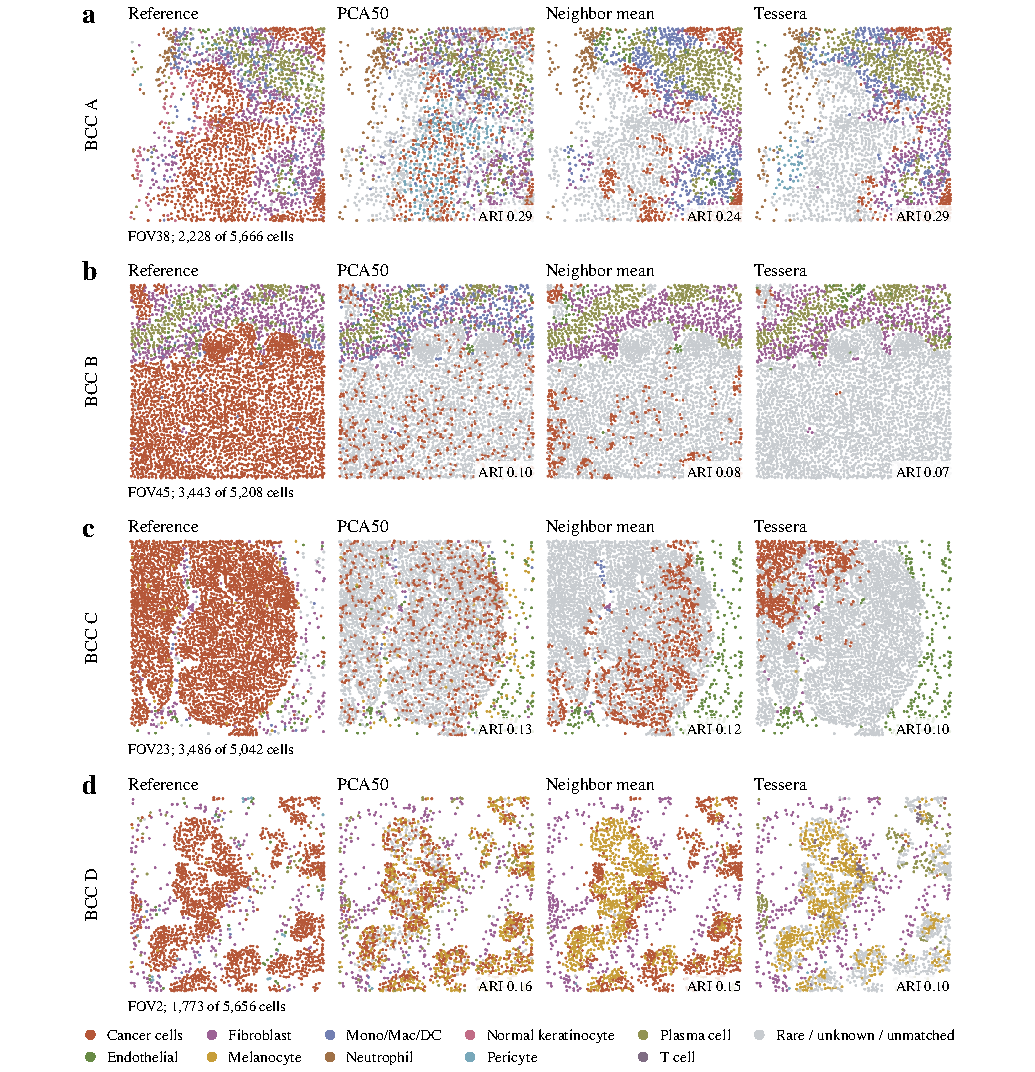
\includegraphics{figure06-bcc-maps.pdf}\end{center}
\noindent{\small Figure 6. BCC display fields. Rows (a--d) show Patients A--D; columns show supplied cell types, PCA50, the six-neighbor mean and Tessera. Seed-1 clusters are matched only to reference classes with at least 1\% object-level prevalence; rare reference classes, unknown labels and unmatched clusters are gray. ARI badges retain original predictions and all valid labels, averaged over three seeds and all retained fields.\par}
\clearpage
\noindent{\Large Tessera\quad Figure 7}\hfill 11 October 2026\par\medskip
\begin{center}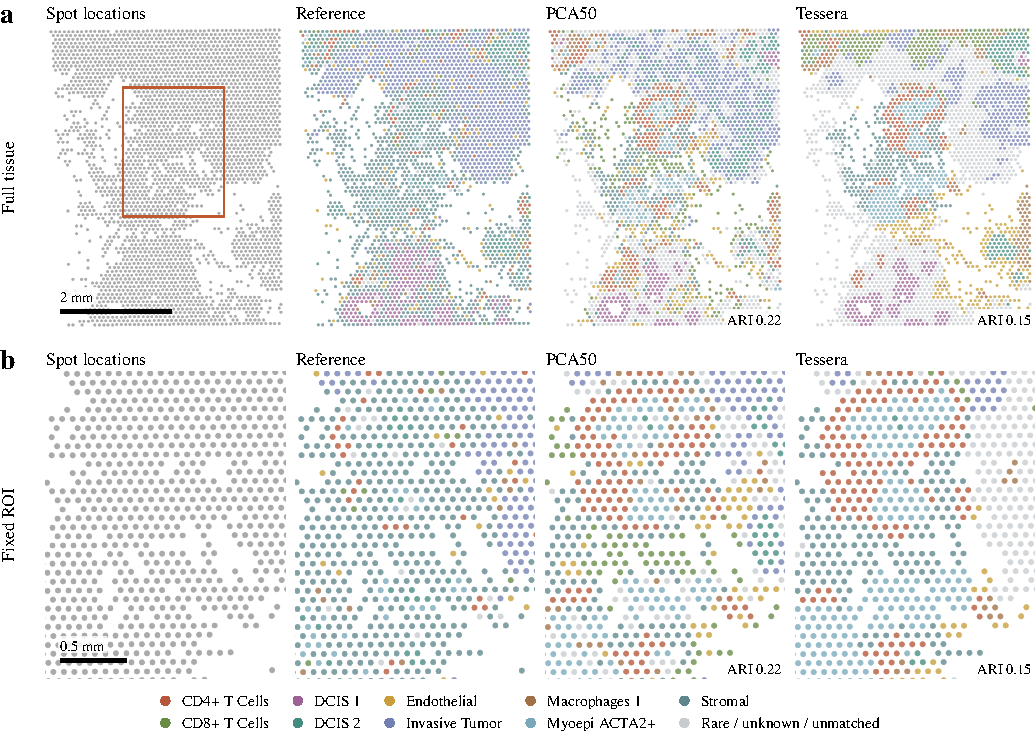
\includegraphics{figure07-breast-histology.pdf}\end{center}
\noindent{\small Figure 7. Breast spatial coordinates and matched representations. Row (a) shows full tissue and row (b) a median-centered ROI with fixed 22\% half-extent, chosen without labels or scores. Columns show measured spot locations, the dominant Xenium-derived reference, PCA50 and Tessera (seed 1). All panels are author-generated coordinate maps; no source histology image is reproduced. Matching excludes reference categories below 1\% object prevalence; rare reference labels, unknowns and unmatched clusters are gray. ARI badges retain all valid classes and are three-seed means. Scale bars use source calibration.\par}
\clearpage
\noindent{\Large Tessera\quad Figure 8}\hfill 11 October 2026\par\medskip
\begin{center}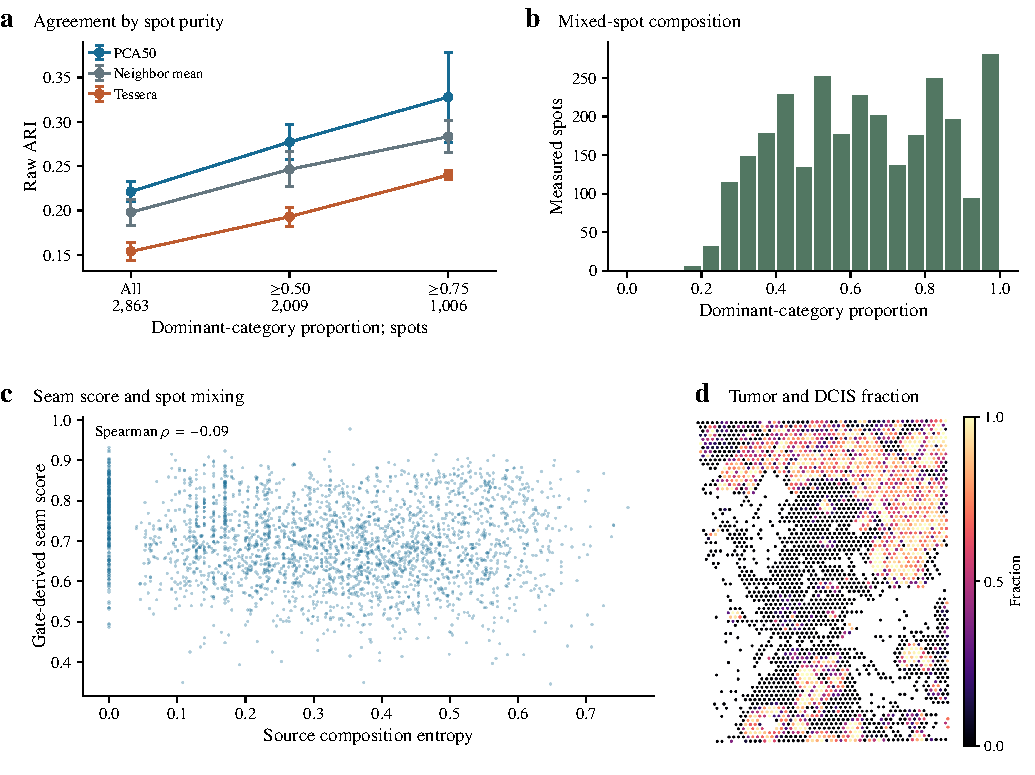
\includegraphics{figure08-breast-mixtures.pdf}\end{center}
\noindent{\small Figure 8. Breast mixed spots. (a) ARI of the fitted partitions when evaluation is restricted to spots whose dominant category exceeds 0.50 or 0.75; error bars are seed SD and the spot counts are under the axis. (b) Distribution of the dominant-category proportion. (c) Gate-derived seam score against source composition entropy (seed 1); a boundary-sensitive score would rise with mixing. (d) Supplied tumor and DCIS fraction per spot.\par}
\clearpage
\noindent{\Large Tessera\quad Figure 9}\hfill 11 October 2026\par\medskip
\begin{center}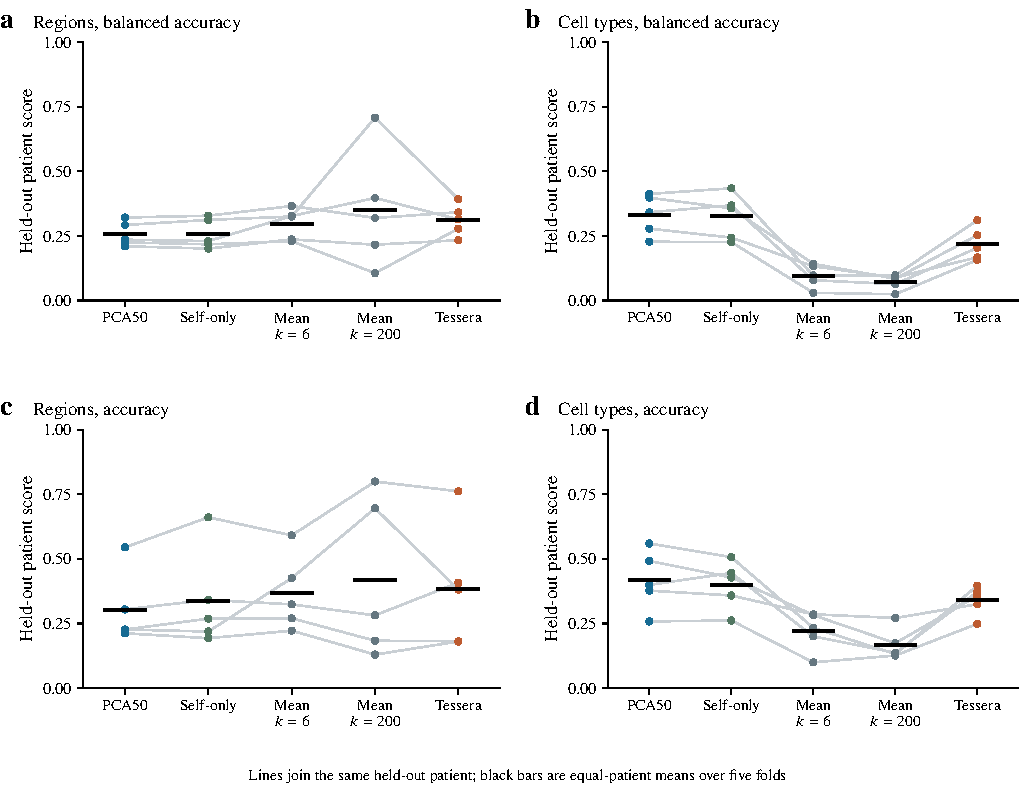
\includegraphics{figure10-patient-transfer.pdf}\end{center}
\noindent{\small Figure 9. Five patient-held-out NSCLC folds. (a, b) Region and cell-type balanced accuracy. (c, d) Accuracy. Four source patients fit scaling, PCA and the encoder; frozen parameters and source-category centroids map the held-out patient. Points are three-seed means for neural arms; fixed neighbor means (\(k=6,200\)) are deterministic descriptive controls, with \(k=200\) informed by earlier lung analyses, not fold-nested tuning. Lines join the same held-out patient; black bars are equal-patient means.\par}
\clearpage
\noindent{\Large Tessera\quad Figure 10}\hfill 11 October 2026\par\medskip
\begin{center}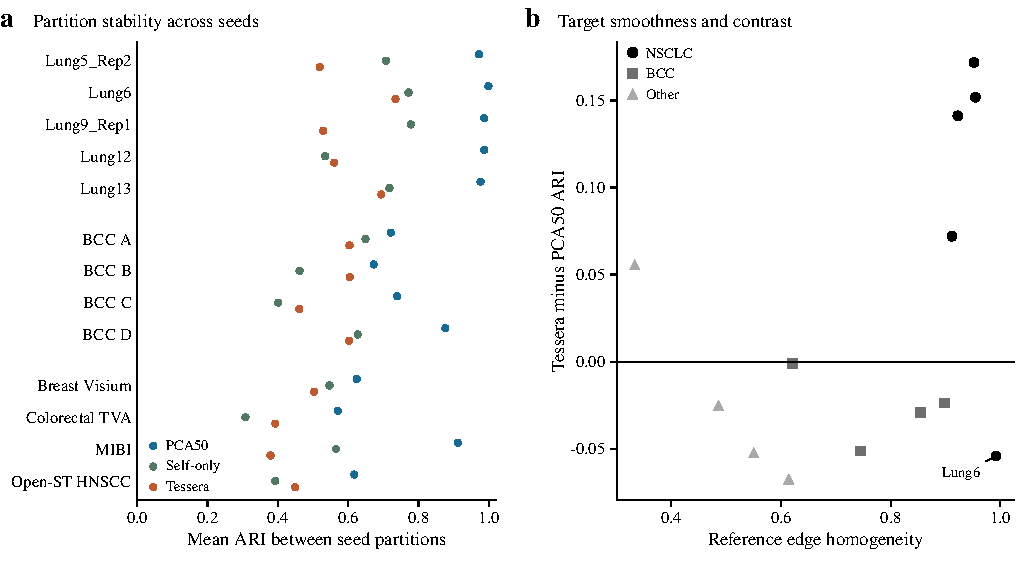
\includegraphics{figure11-stability.pdf}\end{center}
\noindent{\small Figure 10. Optimization stability and target structure. (a) Mean ARI between the three seed partitions on identical inputs. (b) Reference edge homogeneity, the fraction of spatial edges whose endpoints share a supplied label, against the Tessera minus PCA50 contrast. Lung6 is labelled because its high homogeneity reflects a display field dominated by one region.\par}
\clearpage
\noindent{\Large Tessera\quad Figure 11}\hfill 11 October 2026\par\medskip
\begin{center}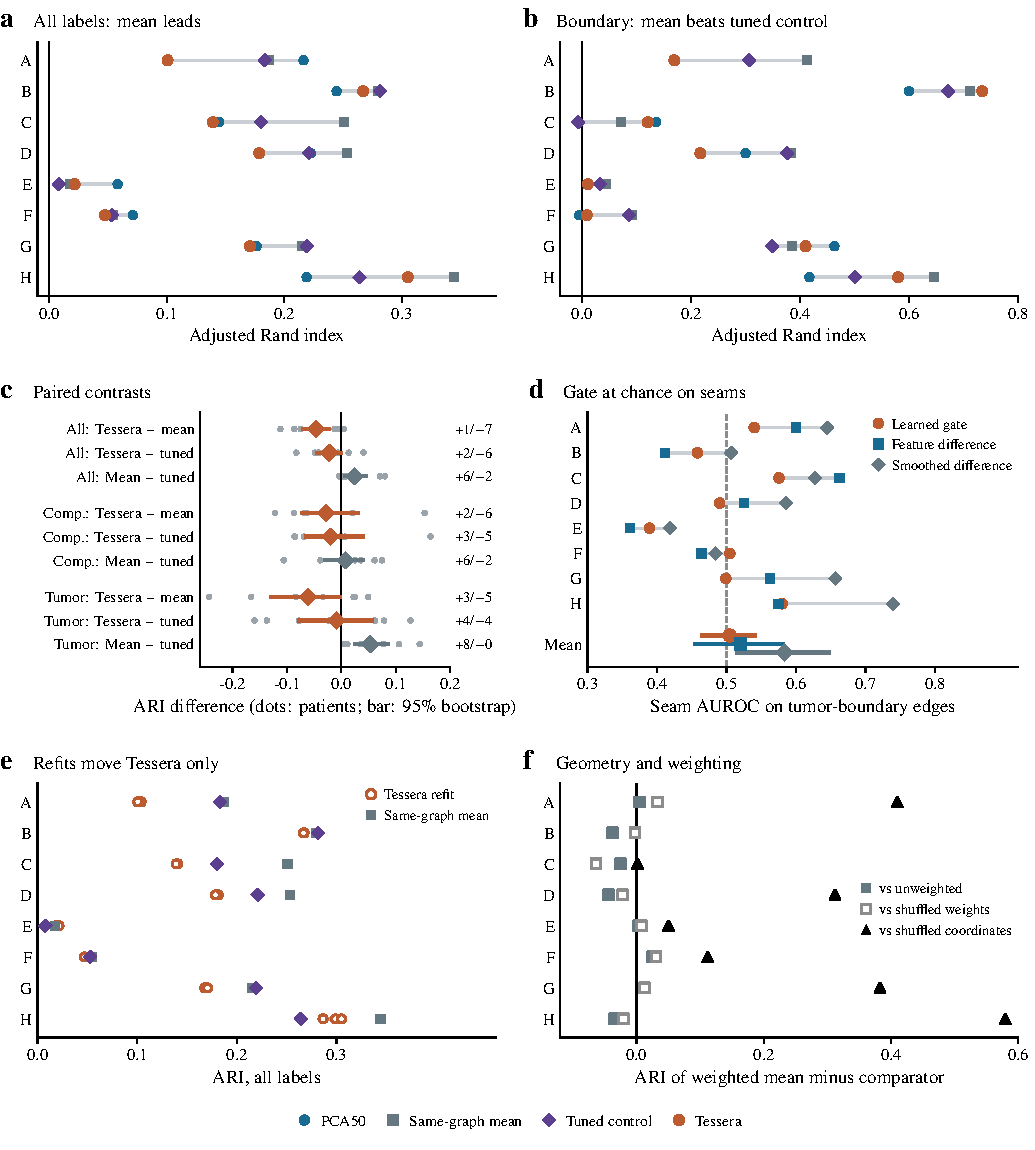
\includegraphics{figure15-external-cohort.pdf}\end{center}
\noindent{\small Figure 11. Independent pathologist-labelled cohort of eight HER2-positive breast tumors; rows A--H are patients. (a, b) Three-seed mean adjusted Rand index for all labels and for the tumor boundary: PCA50, the unweighted mean of neighbors on Tessera's graph, a tuned control selected on the other seven patients, and Tessera. (c) Paired differences for all labels (All), named compartments (Comp.) and the tumor boundary (Tumor); gray dots are patients, diamonds are means with 95\% bootstrap intervals, and the numbers count patients above and below zero. (d) Seam AUROC on tumor-boundary edges for the learned gate, the plain feature difference and the smoothed feature difference; the bottom rows give means with 95\% bootstrap intervals and the dashed line is chance. (e) Tessera's three replicate fits against the same-graph mean and the tuned control, all labels. (f) ARI of the weighted mean minus the unweighted mean, a mean with shuffled weights and a mean with shuffled coordinates, tumor boundary.\par}
\clearpage
\noindent{\Large Tessera\quad Figure 12}\hfill 11 October 2026\par\medskip
\begin{center}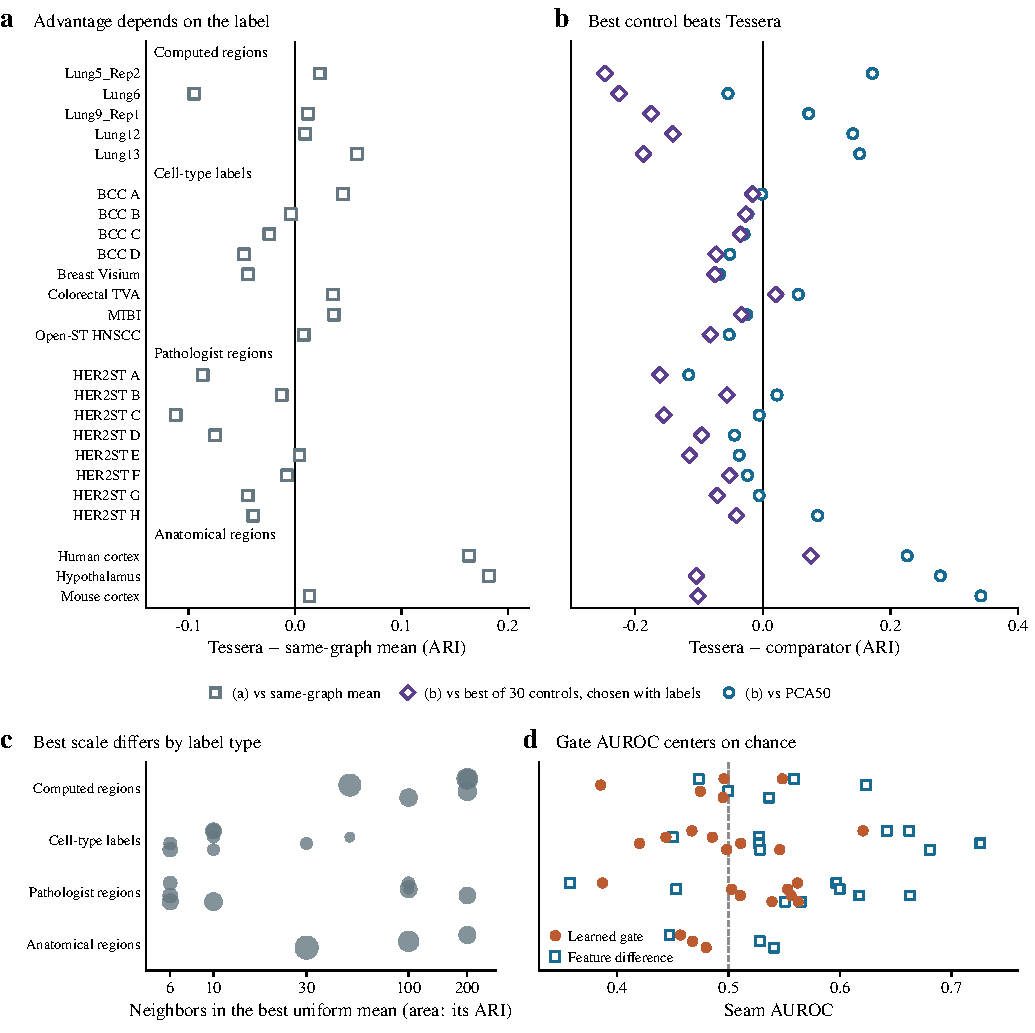
\includegraphics{figure17-tissue-landscape.pdf}\end{center}
\noindent{\small Figure 12. Twenty-four objects grouped by how the annotation was made: the 13 bounded objects, the eight independent patients and three further tissues. (a) Tessera minus the same-graph six-neighbor mean (ARI), which uses no label-based scale selection. (b) Tessera minus the best of 30 simple controls chosen with the test labels (diamonds) and minus PCA50 (circles). (c) Neighborhood size of the best uniform mean for each object; dot area is that mean's ARI. (d) Seam AUROC of the learned gate (filled) and the plain feature difference (open); the dashed line is chance.\par}
\clearpage
\noindent{\Large Tessera\quad Figure S1}\hfill 11 October 2026\par\medskip
\begin{center}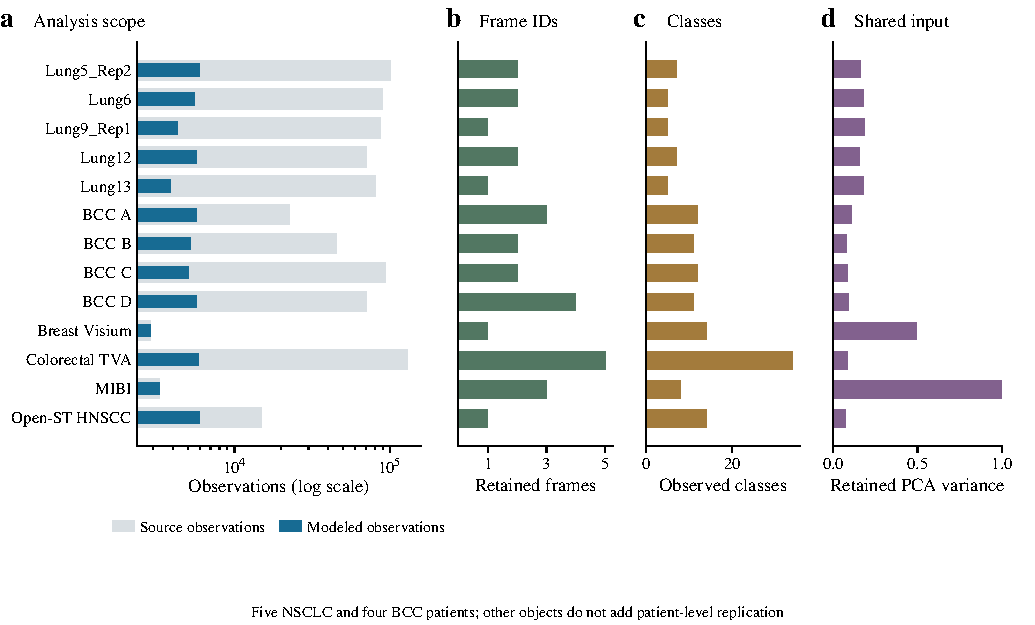
\includegraphics{figure02-cohort.pdf}\end{center}
\noindent{\small Figure S1. Scope of the bounded inputs. (a) Source and modeled observations on a logarithmic axis. (b) Retained coordinate frames. (c) Observed reference classes. (d) Fraction of total variance of the standardized, clipped input retained by the common 50-component PCA.\par}
\clearpage
\noindent{\Large Tessera\quad Figure S2}\hfill 11 October 2026\par\medskip
\begin{center}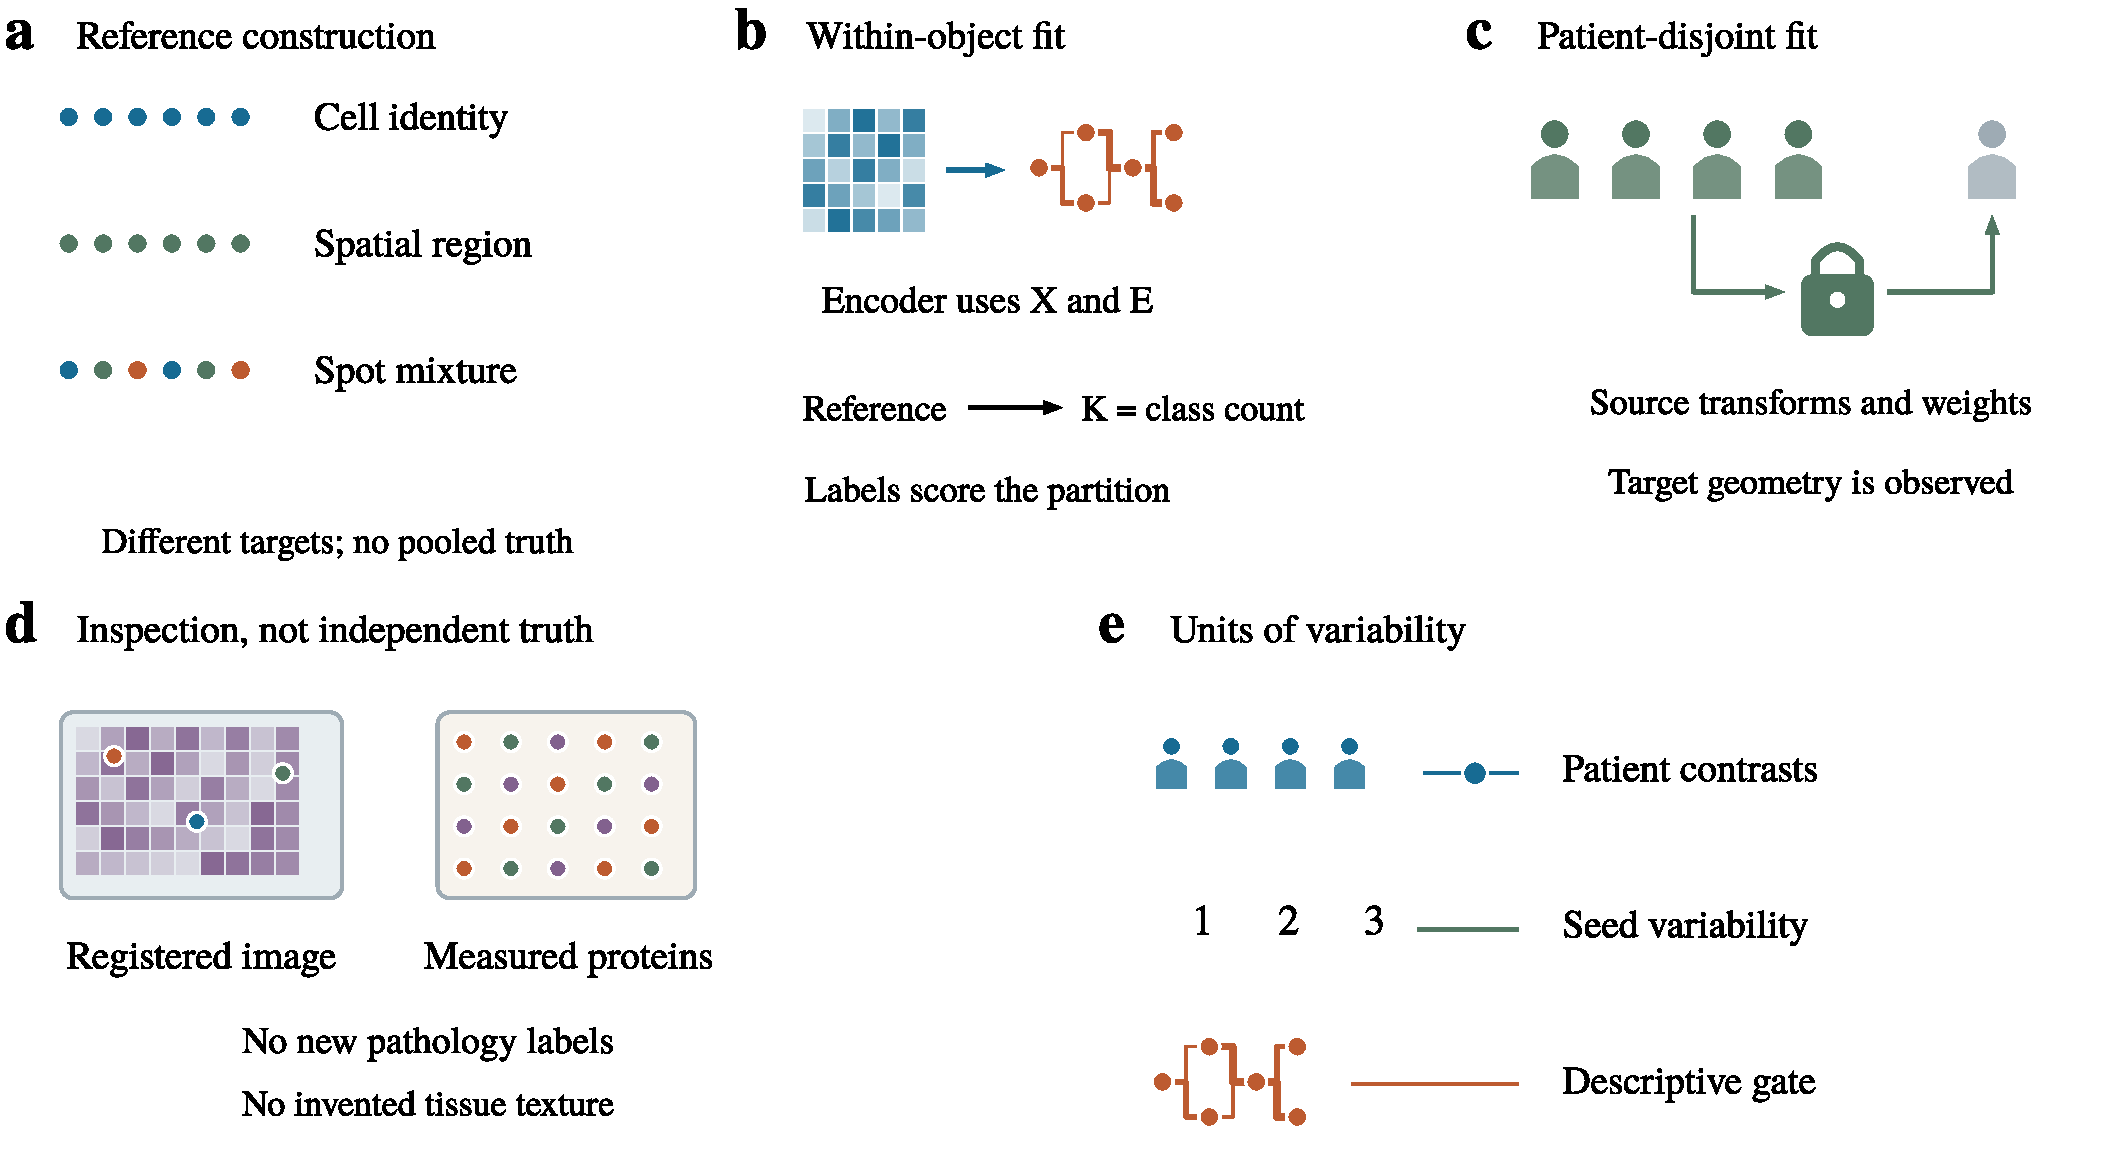
\includegraphics[width=\linewidth,height=.79\textheight,keepaspectratio]{figure14-target-lineage.pdf}\end{center}
\noindent{\small Figure S2. Targets and information access, conceptual. (a) Molecular cell categories, neighborhood-derived regions and mixed-spot compositions come from different constructions. (b) Within-object clustering uses the reference class count but no reference labels. (c) Patient transfer freezes all fitted quantities before the held-out patient is mapped. (d) Registered images and protein channels support inspection only. (e) Patient contrasts, seed variation and gate readouts answer different questions.\par}
\clearpage
\noindent{\Large Tessera\quad Figure S3}\hfill 11 October 2026\par\medskip
\begin{center}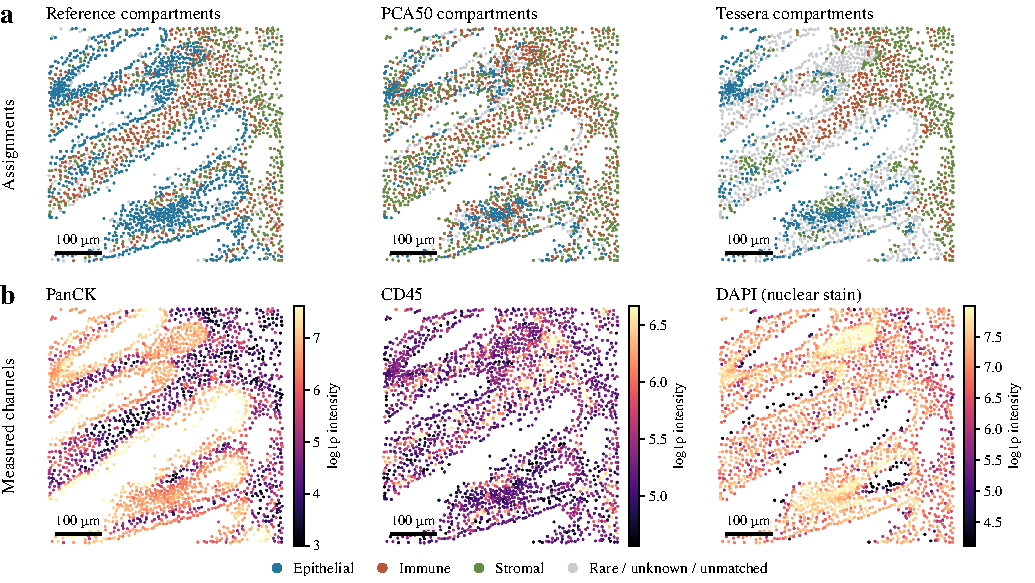
\includegraphics{figure09-colorectal-proteins.pdf}\end{center}
\noindent{\small Figure S3. Colorectal TVA section 232, display field. (a) Supplied compartments and display-matched PCA50 and Tessera assignments; only \texttt{lv2} classes with at least 1\% object prevalence are eligible for matching before modal compartment mapping, and unmatched clusters are gray. (b) Measured PanCK, CD45 and DAPI mean intensities, shown as \(\log(1+x)\) with field-wise 2nd--98th percentile color limits.\par}
\clearpage
\noindent{\Large Tessera\quad Figure S4}\hfill 11 October 2026\par\medskip
\begin{center}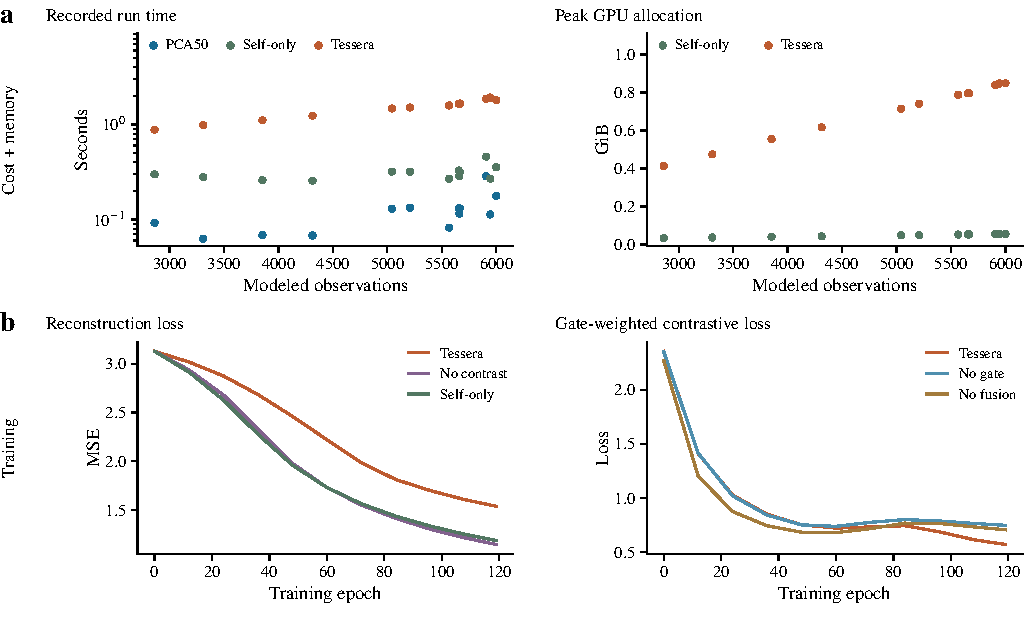
\includegraphics{figure12-efficiency-mechanism.pdf}\end{center}
\noindent{\small Figure S4. Execution and training records. (a) Recorded run time against modeled observations and peak GPU allocation. (b) Reconstruction and gate-weighted contrastive losses for Lung5\_Rep2, seed 1, at the saved epochs.\par}
\clearpage
\noindent{\Large Tessera\quad Figure S5}\hfill 11 October 2026\par\medskip
\begin{center}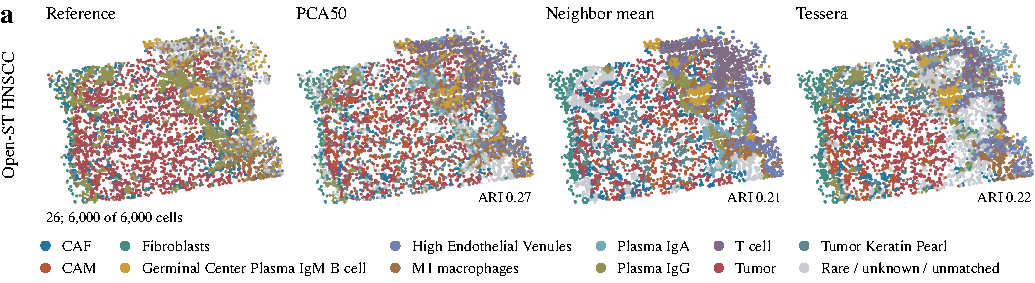
\includegraphics{supplement01-hnscc.pdf}\end{center}
\noindent{\small Figure S5. Open-ST section 26, complete selected 6,000-observation subset. (a) Supplied annotations, PCA50, the six-neighbor mean and Tessera on identical coordinates (seed 1). Matching excludes classes below 1\% object prevalence; rare reference labels, unknowns and unmatched clusters are gray. ARI badges retain original predictions and all valid classes, averaged over three seeds.\par}
\clearpage
\noindent{\Large Tessera\quad Figure S6}\hfill 11 October 2026\par\medskip
\begin{center}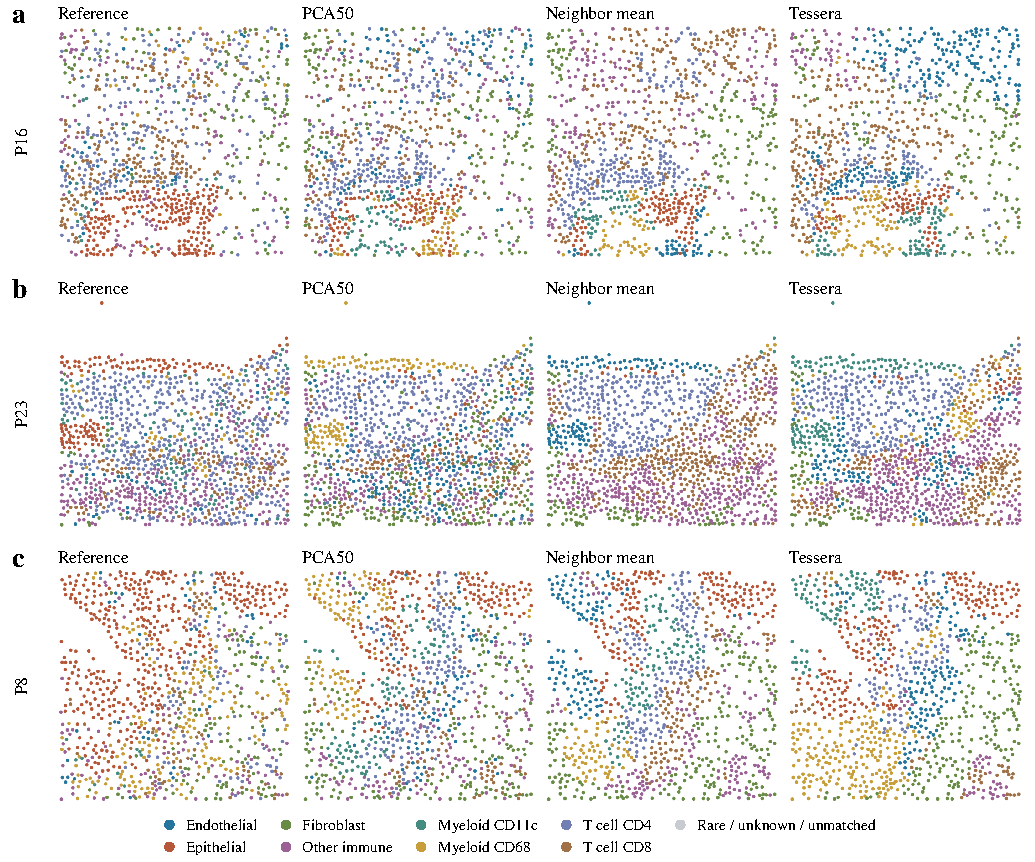
\includegraphics{supplement02-mibi.pdf}\end{center}
\noindent{\small Figure S6. Three MIBI fields in rows (a--c). Columns show supplied molecular categories, PCA50, the six-neighbor mean and Tessera (seed 1). Matching excludes reference classes below 1\% object prevalence; rare reference labels, unknowns and unmatched clusters are gray. Fields are not independent patients.\par}
\clearpage
\noindent{\Large Tessera\quad Figure S7}\hfill 11 October 2026\par\medskip
\begin{center}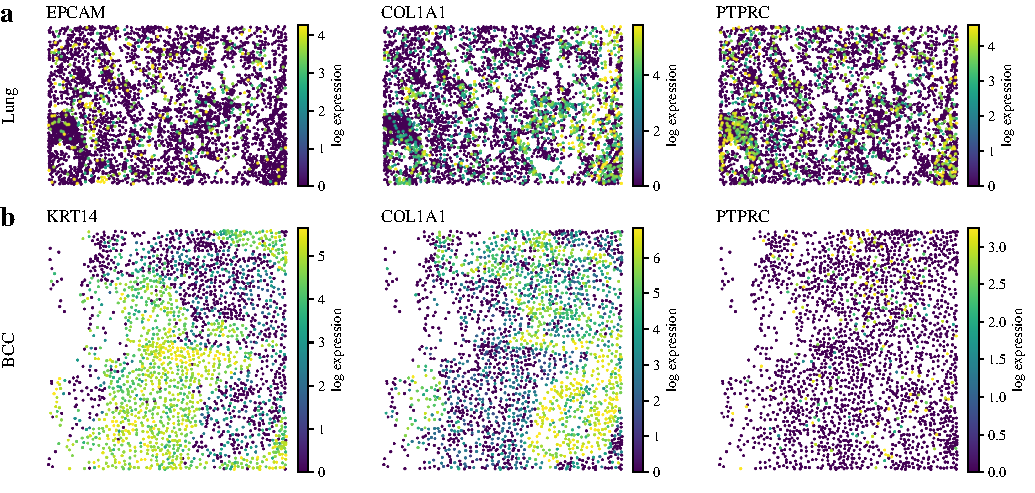
\includegraphics{supplement03-rna-markers.pdf}\end{center}
\noindent{\small Figure S7. Measured RNA markers in the display fields. (a) Lung EPCAM, COL1A1 and PTPRC. (b) BCC KRT14, COL1A1 and PTPRC. Values are the saved log-normalized expression with 0--98th percentile color limits; high-expressing cells are drawn on top.\par}
\clearpage
\noindent{\Large Tessera\quad Figure S8}\hfill 11 October 2026\par\medskip
\begin{center}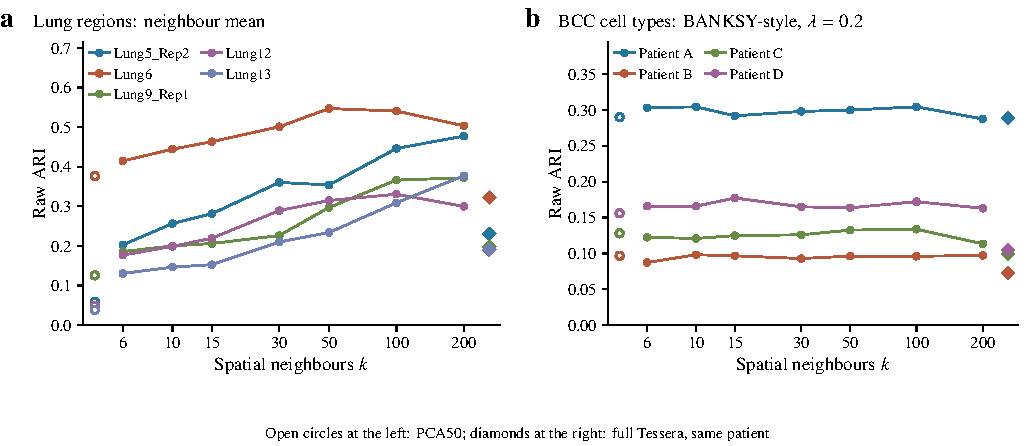
\includegraphics{supplement05-scale-controls.pdf}\end{center}
\noindent{\small Figure S8. Agreement of simple spatial controls as a function of neighborhood size. (a) Lung region ARI of the neighbor mean. (b) BCC cell-type ARI of the BANKSY-style representation with \(\lambda=0.2\). Each line is one patient (three-seed mean); open circles at the left mark PCA50 and diamonds at the right mark full Tessera for the same patient.\par}
\clearpage
\noindent{\Large Tessera\quad Figure S9}\hfill 11 October 2026\par\medskip
\begin{center}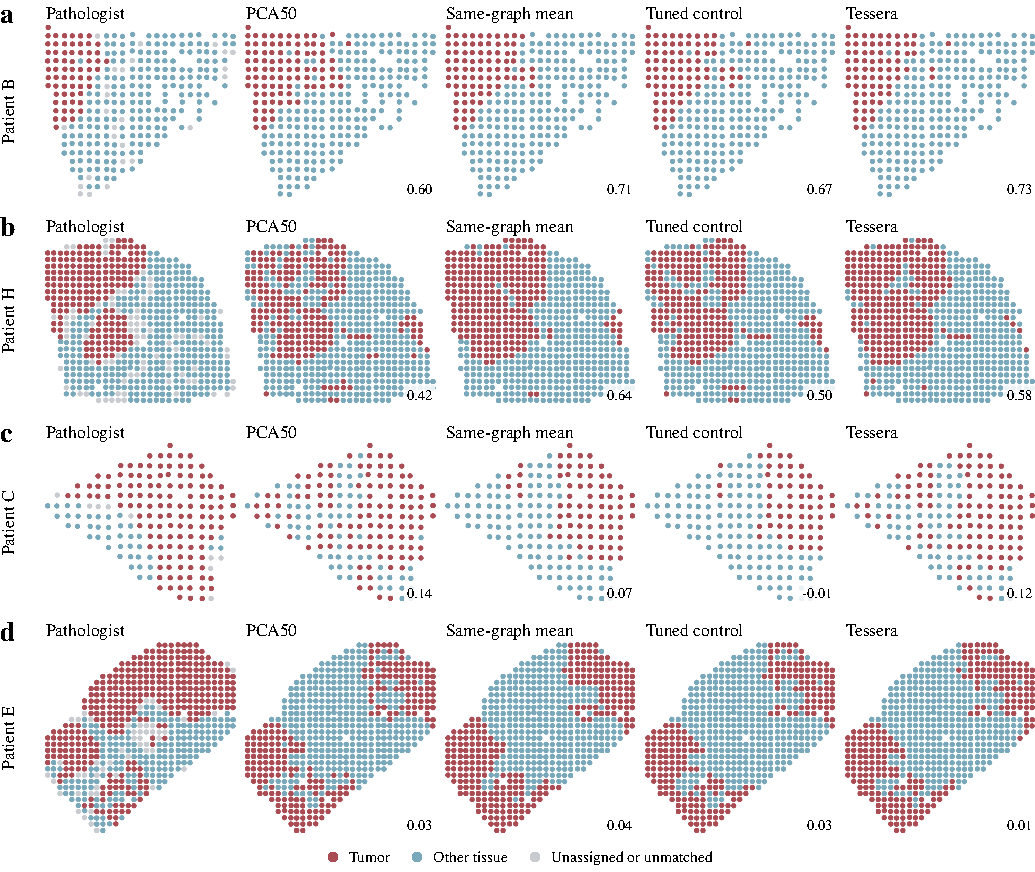
\includegraphics{figure16-external-maps.pdf}\end{center}
\noindent{\small Figure S9. Tumor boundary in four of the eight independent patients: rows (a--d) are the two patients with the highest (B, H) and the two with the lowest (C, E) same-graph mean agreement. Columns show the pathologist's regions, PCA50, the unweighted mean of neighbors on Tessera's graph, a tuned control selected on the other seven patients, and Tessera (seed 1). Clusters are matched to the two classes for display only; gray marks spots the pathologist left unassigned and unmatched clusters. Badges give the three-seed mean ARI against tumor versus other tissue.\par}
\clearpage
\end{document}
